%!TEX program = xelatex

\documentclass[12pt]{article}
\usepackage[UTF8]{ctex}
\usepackage{indentfirst}
\usepackage{lmodern}
\usepackage{setspace}
\usepackage{amsmath}
\usepackage{amssymb}
\usepackage{amsthm}
\usepackage{graphicx}
\usepackage{subfigure}
\usepackage{booktabs}
\usepackage{tabularx}
\usepackage{multirow}
\usepackage{multicol}
\usepackage{listings}
\usepackage{relsize}
\usepackage[usenames]{color}
\usepackage[table]{xcolor}
\usepackage{fontspec}
\usepackage{geometry}
\usepackage{enumitem}
\usepackage{array}
\usepackage{hyperref}
\usepackage{float}

\geometry{left=2.0cm,right=2.0cm,top=2.5cm,bottom=2.5cm}
\graphicspath{{./figures/}}
\onehalfspacing
\setlength{\parindent}{2em}
\addtolength{\parskip}{2pt}
\renewcommand{\arraystretch}{1.35}
\renewcommand\refname{参考资料}

\hypersetup{
    colorlinks=true,
    linkcolor=black,
    urlcolor=blue!60!black
}

\definecolor{lightgray}{RGB}{245,245,244}
\definecolor{deepblue}{RGB}{24,73,133}
\definecolor{softgreen}{RGB}{231,246,238}
\definecolor{softblue}{RGB}{232,242,255}
\definecolor{softorange}{RGB}{255,244,226}
\definecolor{linegray}{RGB}{225,229,235}

\lstset{
    columns=fixed,
    numbers=left,
    numberstyle=\footnotesize\color{gray},
    frame=single,
    rulecolor=\color{linegray},
    backgroundcolor=\color{lightgray},
    keywordstyle=\color{deepblue},
    commentstyle=\it\color[RGB]{0,96,96},
    stringstyle=\rmfamily\slshape\color[RGB]{128,0,0},
    showstringspaces=false,
    breaklines=true,
    basicstyle=\small\ttfamily,
    language=python
}

\setlist[itemize]{itemsep=2pt,topsep=2pt}
\setlist[enumerate]{itemsep=2pt,topsep=2pt}

\newcommand{\code}[1]{{\ttfamily #1}}
\newcolumntype{Y}{>{\raggedright\arraybackslash}X}
\newcolumntype{M}[1]{>{\centering\arraybackslash}p{#1}}
\emergencystretch=3em

\begin{document}

\begin{titlepage}
    \vspace*{-2.4cm}
    \begin{figure}[h]
        \centering
        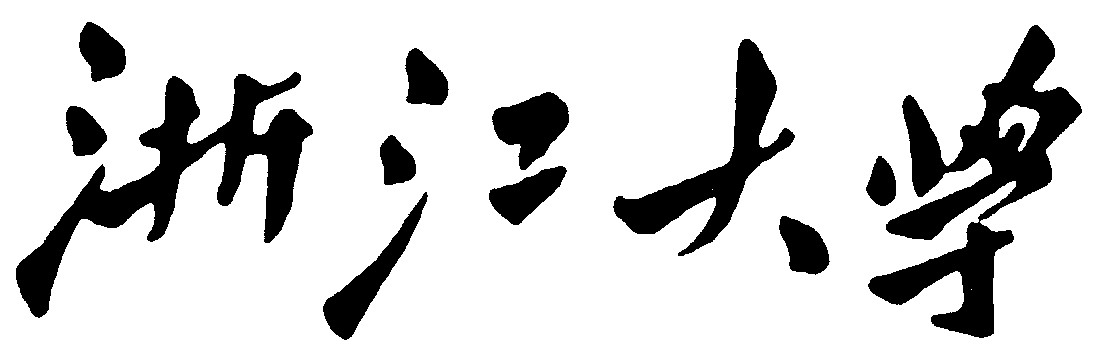
\includegraphics[width=0.8\linewidth]{zjdx}
    \end{figure}
    \begin{figure}[h]
        \centering
        
\includegraphics[width=0.3\linewidth]{qsy}
    \end{figure}
    \vspace{-0.1cm}
    \begin{center}
        \Huge{\textbf{分布式智能物资管理系统}}\\[0.35cm]
        \Large{基于 YOLO 识别、身份门控与本地库存看板的嵌入式项目报告}
    \end{center}
    \vspace*{0.9cm}
    \begin{center}
        \larger[2]{
            \begin{tabular}{cc}
                姓\hspace{12pt}名 & \underline{\makebox[220pt]{\kaishu 黄鹤翔}}\\
                学\hspace{12pt}号 & \underline{\makebox[220pt]{3230106231}}\\
                院\hspace{12pt}系 & \underline{\makebox[220pt]{\kaishu 信息与电子工程学院}}\\
                指导老师 & \underline{\makebox[220pt]{\kaishu 杜歆}}\\
            \end{tabular}
        }
    \end{center}
    \vfill
    \begin{center}
        \large{2026 年 4 月}
    \end{center}
\end{titlepage}

\pagenumbering{arabic}

\section*{摘要}
\addcontentsline{toc}{section}{摘要}

实验室物资借还看似只是登记数量，真正落到现场时却会同时遇到身份确认、拍照时机、数量核对和后续追溯等问题。本项目围绕这一实际场景，完成了一套分布式智能物资管理系统：树莓派或普通 Linux 客户端负责摄像头预览和用户操作，服务端集中运行人脸识别、YOLO 物资计数、TCP 网桥、CSV 记录和本地 Web 看板。系统的一次完整操作由“识别人脸、拍摄操作前物资、用户完成出入库、拍摄操作后物资、自动计算差分并写入记录”组成，最终把识别结果转化为可查询、可解释的库存流水。

与只展示单张图片检测结果的原型不同，本项目更重视闭环可用性。客户端已经脱离 ROS2，改造成独立 Python 包；跨设备通信采用“双长度前缀 + JSON 头 + 二进制图像体”的 TCP 协议，避免客户端配置 DDS 和 ROS2 网络；服务端内部继续使用 ROS2 节点拆分识别任务；库存先写入 \code{server/assets/inventory\_records.csv}，再由本地看板汇总成当前库存、最近操作人和历史详情。当前物资检测模型在 \code{cboard}、\code{dmj4310}、\code{m3508} 三类物资上完成训练验证，第 31 轮达到 mAP50 为 87.74\%、mAP50-95 为 76.15\%，能够支撑课程项目阶段的系统联调和功能展示。

\noindent\textbf{关键词：} 嵌入式系统；物资管理；YOLO；人脸识别；TCP；ROS2；库存看板

\newpage
\tableofcontents
\newpage

\section{项目背景}

小型实验室和机器人队伍常常会共享电机、电调、开发板、相机和传感器。早期用纸质表格或电子表格登记还能应付，但只要借还频率提高，就会出现三个很具体的问题：东西拿走了但忘记补登记，表里写了数量却不知道是谁操作的，记录散落在不同文件里难以追溯。对嵌入式课程项目来说，这些问题又不能简单地靠“上一个复杂后台系统”解决，因为部署环境、开发时间和硬件资源都有限。

因此，本项目没有把目标停在“识别图片里有几个物体”，而是把识别能力嵌入到真实业务动作里。系统需要先知道操作者是谁，再判断操作前后数量变化，最后把变化记录下来并展示出来。这个目标听上去比单点检测朴素，但更接近一个能被实际使用的小型系统。

项目落地时还需要处理两类工程约束。第一，客户端可能部署在树莓派上，图像采集和 UI 应尽量轻，不应强制安装 ROS2 或复杂 GUI 依赖。第二，服务端需要集中管理模型权重、人脸库、记录文件和看板页面，适合保留 ROS2 节点化结构。最后形成的方案是：客户端与服务端之间只走 TCP，服务端内部再用 ROS2 topic 解耦人脸识别和物资识别。

\section{需求与总体思路}

本系统的核心需求可以概括为四条：

\begin{enumerate}
    \item 操作前先完成身份确认，且只接受“恰好一张已知人脸”的结果；
    \item 物资数量不靠用户手填，而是通过操作前后两次图像识别结果自动求差；
    \item 客户端保持轻量，能在树莓派或普通 Linux 环境中直接运行；
    \item 服务端需要能记录每次出入库，并提供一个便于检查结果的本地看板。
\end{enumerate}

围绕这些需求，项目把系统拆成客户端采集控制、网络通信、服务端识别、记录与展示四层。客户端只关心“什么时候拍、把图发给谁、如何提示用户下一步”；服务端负责“识别图像、返回结构化结果、写入库存流水”。这样划分后，各模块的接口比较稳定，调试时也容易定位问题。

\begin{table}[H]
    \centering
    \caption{项目中的主要模块与分工}
    \label{tab:modules}
    {\small
    \begin{tabularx}{\textwidth}{M{2.2cm}M{5.4cm}Y}
        \toprule
        层次 & 关键文件或节点 & 作用 \\
        \midrule
        客户端采集 & \code{camera\_node.py}、\code{camera\_backend.py} & 优先调用 \code{rpicam-still} 采集 JPEG，环境不支持时回退到 OpenCV。 \\
        客户端流程 & \code{logic\_node.py}、\code{ui\_node.py} & 用状态机管理人脸识别、手动前态抓拍、完成按钮、后态抓拍和差分上传。 \\
        网络协议 & \code{tcp\_client\_node.py}、\code{tcp\_bridge\_node.py}、\code{tcp\_protocol.py} & 用双长度前缀传输“UTF-8 JSON 头 + 可选二进制图像体”，默认图片格式改为 \code{webp} 以降低带宽占用。 \\
        服务端识别 & \begin{tabular}[c]{@{}c@{}}\code{face\_recognize\_node.py}\\\code{material\_counter\_node.py}\end{tabular} & 分别完成人脸识别和 YOLO 物资计数，并通过 ROS2 topic 返回 JSON。 \\
        记录展示 & \begin{tabular}[c]{@{}c@{}}\code{inventory\_records.csv}\\\code{inventory\_web\_node.py}\end{tabular} & 将出入库流水落盘，并在 \code{127.0.0.1:8600} 汇总展示库存状态。 \\
        \bottomrule
    \end{tabularx}
    }
\end{table}

\section{技术路线与选型依据}

本项目涉及的技术点比较多，但它们并不是孤立堆叠的。整体原则是：客户端尽量轻，服务端集中推理；跨设备边界保持简单，服务端内部再用节点化方式拆分复杂任务；识别结果必须能进入库存流水，而不是只停留在画框展示。表~\ref{tab:tech-principles} 先概括各技术点的基本原理和采用理由。

\begin{table}[H]
    \centering
    \caption{关键技术点的原理和选型理由}
    \label{tab:tech-principles}
    {\small
    \begin{tabularx}{\textwidth}{M{2.4cm}Y Y}
        \toprule
        技术点 & 基本原理 & 本项目采用理由与优势 \\
        \midrule
        ROS2 节点通信 & ROS2 把功能拆成多个节点，节点之间通过 topic、service 或 action 交换消息。发布者和订阅者只依赖消息类型，不直接依赖彼此实现。 & 推理任务集中在服务端，适合用 ROS2 管理人脸识别、物资识别、TCP 网桥和看板节点。模块可以单独启动、单独替换，服务端最大单文件从旧版 \code{integrated\_server.py} 的 725 行下降到当前最大服务端节点 355 行。 \\
        TCP 长连接 & TCP 提供可靠、有序的字节流。由于字节流本身没有消息边界，项目用 4 字节 JSON 长度和 4 字节二进制长度标明每条消息的头部与附件范围。 & 客户端不需要安装 ROS2，也不用处理 DDS 发现和跨网段配置；只要能发送压缩图片和 JSON 头就能接入服务端。当前协议只暴露 \code{face\_image}、\code{material\_image}、\code{inventory\_record} 三类请求，边界清楚。 \\
        YOLO 检测 & YOLO 是单阶段目标检测方法，直接从整张图中预测目标框、类别和置信度。项目把同类检测框累加，得到每类物资数量。 & 相比逐个扫描二维码，YOLO 更适合“拍一张货架图后统计类别数量”。当前三类物资在第 31 轮达到 Precision 80.21\%、Recall 80.36\%、mAP50 87.74\%，已能支撑系统闭环演示。 \\
        人脸识别门控 & \code{face\_recognition} 会把人脸转为特征编码，再用距离阈值与已知人脸库比较。距离越小，越可能是同一人。 & 库存记录必须绑定责任人。本项目要求画面中恰好一张已知人脸，才允许进入物资操作阶段，避免“未知人员”或“多人同时入镜”导致责任归属不清。 \\
        有限状态机 & 状态机把流程拆成有限个状态，每个状态只允许特定输入和转移。UI 按钮状态由当前状态决定。 & 出入库动作天然有顺序：身份确认、前态拍摄、用户操作、后态拍摄、差分提交。状态机让用户不容易跳步，也让异常重试和超时处理更明确。 \\
        CSV 与本地看板 & CSV 是追加式文本记录；Web 看板再周期性读取 CSV，聚合库存、最近事件和低库存状态。 & 课程项目阶段并发低、调试频繁，CSV 便于直接检查；看板补足展示能力，让老师或同学不用打开代码也能确认系统是否真正写入了库存流水。 \\
        \bottomrule
    \end{tabularx}
    }
\end{table}

为了避免“看起来合理但没有依据”的选型说明，表~\ref{tab:evidence} 汇总了仓库中可以直接核对的工程数据。部分指标不是严格性能测试，但能说明实现规模、部署成本和模型效果的变化方向。

\begin{table}[H]
    \centering
    \caption{支撑技术选型的项目数据}
    \label{tab:evidence}
    {\small
    \begin{tabularx}{\textwidth}{M{3.6cm}M{4.4cm}Y}
        \toprule
        指标 & 数值 & 说明 \\
        \midrule
        早期主线迭代次数 & \code{main} 分支 15 次提交 & 记录了从人脸、TCP、二维码到完整客户端/服务端和 YOLO 框架的演进。 \\
        客户端第三方 Python 依赖 & 2 个：\code{numpy}、\code{opencv-python} & UI 使用标准库 \code{tkinter}，相机优先走 \code{rpicam-still}，因此客户端部署负担较小。 \\
        当前 TCP 请求类型 & 3 类 & 分别对应身份识别、物资计数和库存记录，协议面没有暴露服务端内部 ROS2 细节。 \\
        数据集实际图像数量 & 61 张 & 训练/验证/测试集分别为 36/18/7 张，覆盖 \code{cboard}、\code{dmj4310}、\code{m3508} 三类物资。 \\
        较优训练指标 & mAP50 87.74\%，mAP50-95 76.15\% & 来自训练结果 CSV 中的第 31 轮记录。 \\
        图像上传改造效果 & 平均 TCP 报文从 2.47 MB 降到 0.37 MB & 基于 11 张物资验证图和 2 张已知人脸图的实测，旧方案为 \code{base64+jpeg}，新方案为 \code{binary+webp}，平均降幅 84.53\%。 \\
        单文件压力变化 & 服务端 725 行降至 355 行；客户端 533 行降至 398 行 & 对比旧版 \code{main} 分支的单体文件和当前最大模块文件，说明职责拆分后单个文件更容易阅读和维护。 \\
        \bottomrule
    \end{tabularx}
    }
\end{table}

除了“协议边界更清楚”之外，图像编码方式本身也直接影响分布式部署时的带宽占用。旧版客户端将 \code{jpeg} 字节流先做 \code{base64}，再嵌入 JSON；这样虽然实现简单，但会把图片体积额外放大约三分之一，而且服务端面对多条 TCP 长连接时，大部分流量都被字符串化图像占据。新版实现改成“JSON 头 + 二进制图像体”：JSON 头只保留 \code{request\_id}、\code{image\_format} 和字节长度，真实图像作为独立二进制附件发送，默认编码则调整为 \code{webp} 质量 75。这里优化的是 \emph{TCP 上传阶段}，并不改变服务端识别接口的业务语义。

表~\ref{tab:encoding-benchmark} 给出了仓库内实际样本的对比数据。测试样本包含 \code{datasets/materials/images/val} 中可正常读取的 11 张物资图，以及 \code{server/assets/known\_face/} 中 2 张已知人脸图。旧方案按“\code{jpeg} 质量 90 + \code{base64} + 单长度头”计算总报文大小；新方案按“\code{webp} 质量 75 + 二进制附件 + 双长度头”计算。结果表明，两类场景的平均报文大小都下降到了原来的约五分之一到六分之一。

\begin{table}[H]
    \centering
    \caption{旧图像编码与新图像编码的 TCP 报文大小对比}
    \label{tab:encoding-benchmark}
    {\small
    \begin{tabularx}{\textwidth}{M{2.8cm}M{1.4cm}M{2.6cm}M{2.6cm}M{1.8cm}Y}
        \toprule
        样本类型 & 样本数 & 旧方案平均报文 & 新方案平均报文 & 平均降幅 & 说明 \\
        \midrule
        物资识别图像 & 11 & 2.43 MB & 0.37 MB & 85.22\% & 样本来自物资验证集，分辨率高、背景复杂，更接近货架计数场景。 \\
        人脸识别图像 & 2 & 2.66 MB & 0.39 MB & 80.76\% & 样本来自已登记人脸库，人物构图集中，但原始分辨率差异较大。 \\
        合并平均 & 13 & 2.47 MB & 0.37 MB & 84.53\% & 新方案在同一批样本上显著减小了跨设备传输流量。 \\
        \bottomrule
    \end{tabularx}
    }
\end{table}

从编码结构看，降幅的主要来源有两点。第一，旧方案的 JSON 体平均达到 2.47 MB，而新方案的 JSON 头在同一批样本上平均仅 161 B，说明把图像从 JSON 中剥离出来本身就消除了大部分冗余；第二，\code{webp} 在这些样本上的平均图像体积约为 0.37 MB，也明显小于旧方案中平均 1.85 MB 的 \code{jpeg} 字节流。因此，这次改动不仅降低了单次请求带宽，也更有利于服务端在多 TCP 连接并发时维持稳定吞吐。

\section{系统总体结构}

图~\ref{fig:system-arch-gpt} 是根据当前仓库模块生成的系统总体结构图。图中英文标签对应代码中的真实类名或节点名，便于和工程文件互相对照。

\begin{figure}[H]
    \centering
    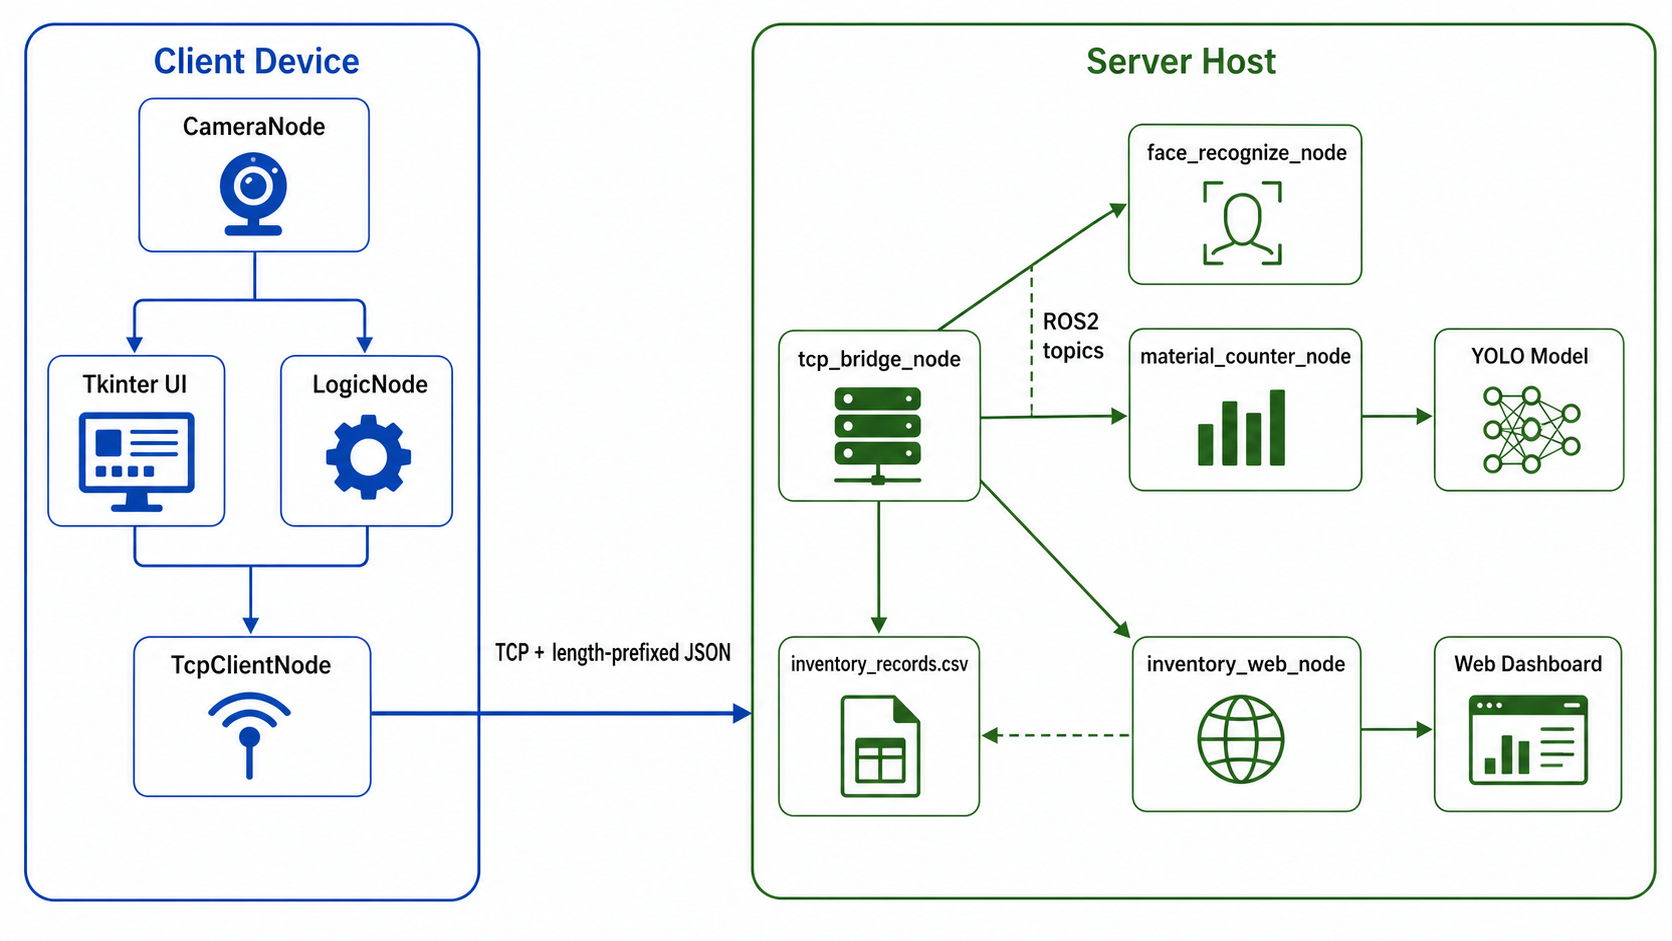
\includegraphics[width=0.98\textwidth]{system_architecture_gpt_image2}
    \caption{系统总体结构图（gpt-image2 生成，按项目模块整理）}
    \label{fig:system-arch-gpt}
\end{figure}

从架构上看，客户端和服务端的边界非常清楚。客户端侧包含 \code{CameraNode}、\code{Tkinter UI}、\code{LogicNode} 和 \code{TcpClientNode}。其中 \code{CameraNode} 负责持续维护最新画面，\code{LogicNode} 根据业务状态决定何时抓拍并发送请求，\code{TcpClientNode} 复用 TCP 连接向服务端提交 \code{face\_image}、\code{material\_image} 和 \code{inventory\_record} 三类请求。

服务端侧以 \code{tcp\_bridge\_node} 为入口。它对外监听 TCP，对内把图片转成 ROS2 的 \code{sensor\_msgs/msg/Image} 发布到识别节点；人脸识别和物资识别结果再以 \code{std\_msgs/msg/String} 中的 JSON 返回。库存记录不进入模型节点，而是由 TCP 网桥在校验请求后直接追加到 CSV 文件。Web 看板节点轮询同一份 CSV，构建当前库存、低库存提示、最近事件和单物资详情。

这种结构的好处不在于技术栈堆得多，而在于每层的压力被放在了合适的位置：树莓派只做采集和交互，服务器负责推理和汇总；客户端不用安装 ROS2，服务端又能保留 ROS2 对识别模块的组织能力。

\section{项目运行流程}

系统一次出入库操作的主链路如图~\ref{fig:workflow-gpt} 所示。这里最重要的设计是“先身份、再前态、再后态、最后差分”，而不是在操作过程中连续猜测用户是否已经拿取完成。

\begin{figure}[H]
    \centering
    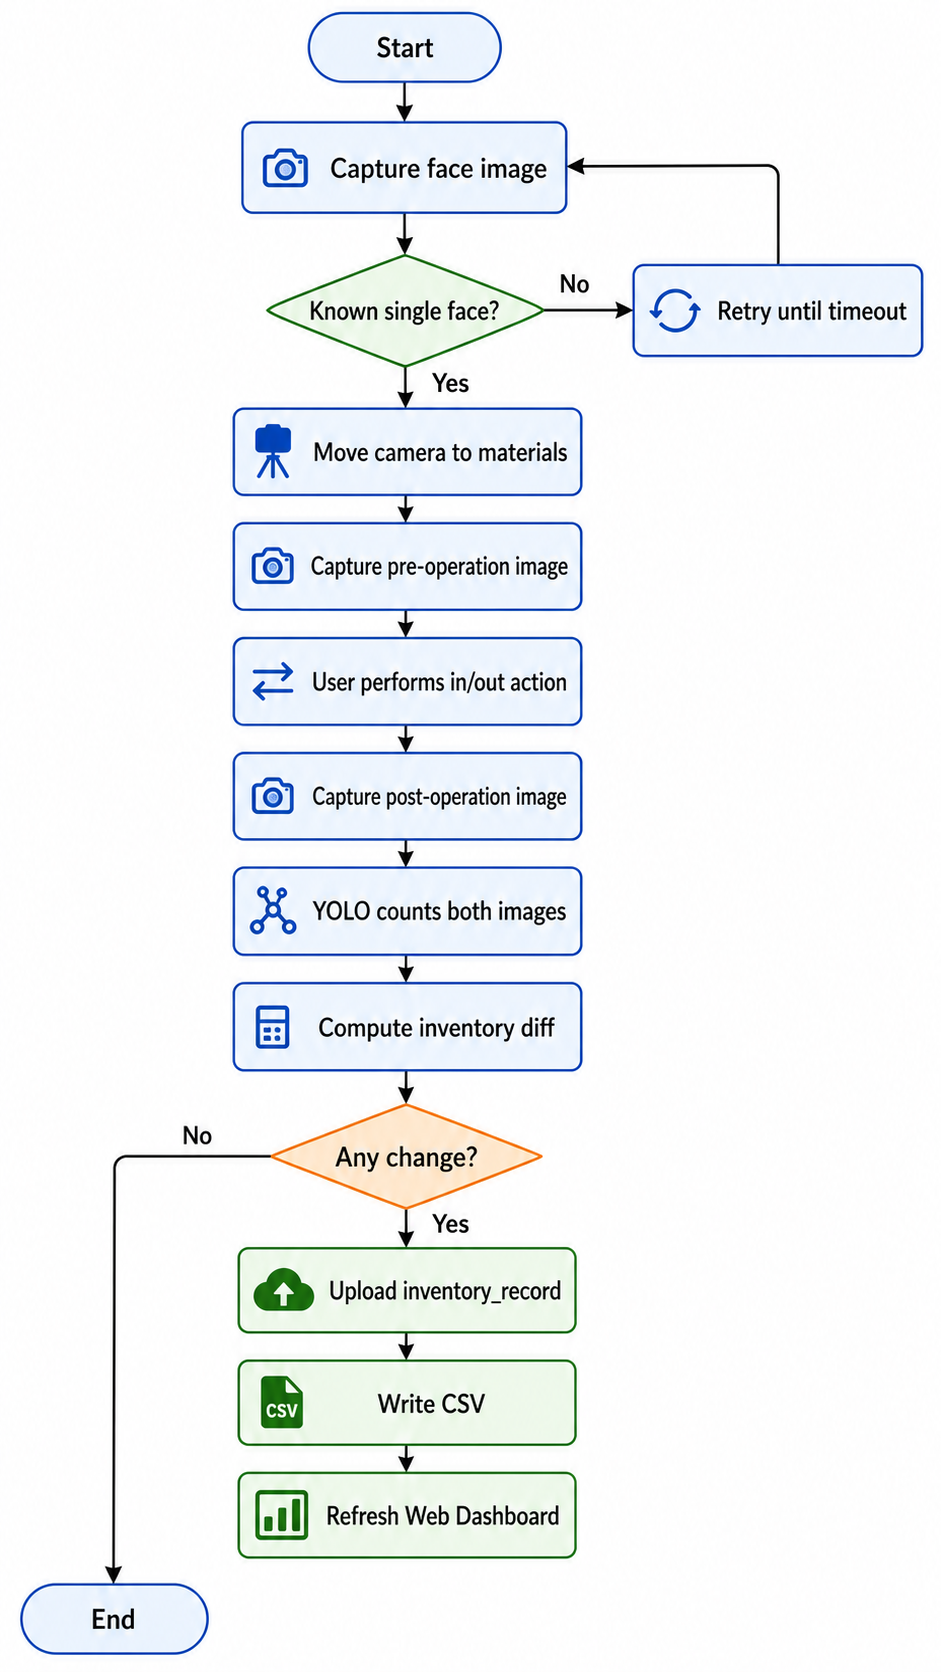
\includegraphics[width=0.68\textwidth]{project_workflow_gpt_image2}
    \caption{项目主流程图（gpt-image2 生成，结合客户端状态机整理）}
    \label{fig:workflow-gpt}
\end{figure}

客户端初始状态为 \code{idle}。用户点击 Start 后，状态切换到 \code{recognizing\_face}，程序每隔约 1 秒抓拍人脸图并发给服务端。只有当返回结果中 \code{total\_faces=1}，且唯一人脸名称不是 \code{unknown} 时，系统才记录操作者姓名并进入 \code{waiting\_camera\_move}。如果画面里没人、多人或未知人员，流程会继续重试直到超时。

识别通过后，用户把摄像头对准物资区域并点击 \code{Capture Materials}。这一步是项目后期专门调整过的：早期尝试用画面稳定性自动判断前态抓拍时机，但在移动摄像头和现场遮挡时误差较大，因此改为手动触发。该选择牺牲了一点自动化，但显著降低了误拍概率，也让演示流程更可控。

前态计数保存后，用户完成真实出入库操作并点击 Finish，客户端再拍摄后态图像。两次 \code{material\_image} 返回后，\code{compute\_inventory\_changes()} 对两份计数字典逐项求差。正差生成“入库”记录，负差生成“出库”记录；若差分为空，流程直接结束，不写入无意义流水。

\section{关键实现}

\subsection{轻量客户端与状态机}

客户端现在是一个独立 Python 包，入口由 \code{client/pyproject.toml} 暴露，常用命令包括 \code{embedded-client}、相机检查入口和服务端连通性检查入口。它的技术原则是“端侧只保留必要交互”：摄像头负责取图，UI 负责显示和按钮，网络模块负责发请求，业务状态机决定下一步动作。这样做可以把树莓派上的环境压力控制住，当前客户端第三方依赖只有 \code{numpy} 和 \code{opencv-python} 两项，界面使用 Python 标准库里的 \code{tkinter}。

相机后端采用自动选择策略。若环境中存在 \code{rpicam-still}，系统会用命令行直接输出 JPEG 到标准输出并在内存中解码；否则回退到 OpenCV 摄像头。选择 \code{rpicam-still} 的原因是树莓派新系统中它比直接打开 OpenCV 摄像头更稳定，回退路径则保证了普通 USB 摄像头也能用于开发调试。

流程控制使用有限状态机。有限状态机的优点是每个阶段只开放当前合理的操作，例如人脸识别未通过时不能提交库存，前态未拍摄时不能点击 Finish。当前 \code{LogicNode} 的关键状态包括 \code{recognizing\_face}、\code{waiting\_camera\_move}、\code{capturing\_pre\_material}、\code{waiting\_finish}、\code{capturing\_post\_material}、\code{computing\_diff} 和 \code{submitting\_inventory}。相比旧版把 UI、相机、舵机和网络逻辑混在 \code{smart\_client.py} 的做法，现在最大客户端模块为 398 行，低于旧版客户端单文件 533 行，代码职责也更容易定位。

\subsection{TCP 协议与跨设备边界}

TCP 是面向连接的可靠字节流协议，适合在局域网内传输图像请求和结构化结果。但 TCP 只保证字节顺序，不保证“一次发送对应一次接收”，因此协议必须自己定义消息边界。本项目采用 4 字节大端长度前缀加 UTF-8 JSON 的格式：接收端先读固定 4 字节得到消息长度，再按长度读取完整 JSON。这样既避免粘包拆包问题，又保持消息内容便于调试。

跨设备通信没有采用跨机器 ROS2，是因为 ROS2 的 DDS 发现机制在多网卡、校园网或树莓派网络环境中经常需要额外配置。项目把 ROS2 留在服务端内部，把客户端和服务端之间的边界收敛为 TCP，就把部署要求降到了“能连上 IP 和端口”。图片在客户端压缩为 JPEG 后转成 Base64 放入 JSON，服务端再解码成 OpenCV 图像；对课程项目而言，这比二进制私有协议更容易排错。

\begin{lstlisting}[language={},caption={库存记录请求示例},label={lst:inventory-json}]
{
  "type": "inventory_record",
  "request_id": "req-002",
  "payload": {
    "time": "2026-04-25T21:30:00+08:00",
    "person": "huanghexiang",
    "action": "出库",
    "items": [
      {"name": "cboard", "quantity": 2},
      {"name": "m3508", "quantity": 1}
    ]
  }
}
\end{lstlisting}

服务端支持三类请求：\code{face\_image}、\code{material\_image} 和 \code{inventory\_record}。其中前两类会被转发到识别节点，后一类会经过字段校验后写入 CSV。协议层还处理了 \code{INVALID\_JSON}、\code{INVALID\_IMAGE}、\code{INVALID\_INVENTORY}、\code{TIMEOUT} 等错误码，便于客户端给出明确失败原因。

\subsection{ROS2 服务端节点}

ROS2 的核心价值是把功能拆成节点，再用消息把节点连接起来。本项目服务端保留 ROS2 Humble 包结构，核心 launch 文件是 \code{tcp\_bridge.launch.py}，会同时启动物资识别、人脸识别、TCP 网桥和 Web 看板。TCP 网桥把外部请求转成 ROS2 图像消息，识别节点只订阅图像并发布 JSON 结果；库存记录和看板不直接依赖模型内部实现。

这种拆分的理由有两个。第一，服务端更适合集中安装模型库、ROS2 和人脸识别依赖，硬件资源也比客户端宽裕。第二，节点化可以降低单个文件的维护压力：旧版 \code{integrated\_server.py} 有 725 行，当前最大服务端节点 \code{tcp\_bridge\_node.py} 为 355 行，人脸、物资、看板分别落在独立文件中。代码总量并没有简单减少，因为系统功能增加了；但单个模块的职责更清楚，替换某个识别节点时不需要重写整个服务端。

\subsection{YOLO 物资检测}

YOLO 属于单阶段目标检测方法，它不先生成候选区域，而是直接在一次前向推理中预测目标框、类别和置信度。项目使用这种方法的原因，是物资管理更关心“画面中每类物资有几个”，不一定需要知道每个物体的唯一编号。识别节点收到图像后调用模型推理，再按类别累加检测框数量，最终返回类似 \code{\{"cboard": 2, "m3508": 1\}} 的计数字典。

物资识别节点默认通过 \code{resolve\_default\_model\_path()} 查找权重，优先使用材料模型目录下的 \code{last.pt}，找不到时回退到 \code{best.pt}。这样部署时可以直接使用最新训练产物，同时保留按 mAP 选出的评估权重。当前模型在三类物资上第 31 轮达到 Precision 80.21\%、Recall 80.36\%、mAP50 87.74\%、mAP50-95 76.15\%。这些指标不是生产级大数据结论，但足以说明在现有小数据集上，YOLO 路线已经可以支持前后态差分演示。

\subsection{人脸识别门控}

人脸识别使用 \code{face\_recognition} 库。它的基本思路是先检测人脸位置，再把人脸转为向量编码，最后计算待识别人脸与已知人脸编码之间的距离；距离低于阈值时，认为两者更可能属于同一人。节点启动时读取 \code{server/assets/known\_face/}，为已登记人员生成编码；运行时默认匹配阈值为 \code{0.45}，检测模型为 \code{hog}。

在本系统中，人脸识别不追求复杂的人事管理，而是承担流程门控职责。客户端只有在服务端返回 \code{total\_faces=1} 且唯一姓名不是 \code{unknown} 时才继续。这一规则比“识别到某个人就放行”更严格，可以过滤无人、多人和未知人员三类不可靠场景。它的优越性体现在库存记录上：每条流水都有明确操作者，后续追溯不需要再靠口头确认。

\subsection{库存记录与看板}

库存记录的原理比较朴素：把一次差分结果拆成多条追加式流水，每一行都包含操作者、动作、物资名和数量。字段包括 \code{request\_id}、\code{record\_time}、\code{person}、\code{action}、\code{material\_name}、\code{quantity} 和 \code{received\_at}。CSV 方案虽然不适合高并发生产环境，但对课程项目非常实用：文件可直接打开检查，出错时也容易定位是哪一次请求写入了哪几行。

Web 看板由 \code{inventory\_web\_node.py} 提供，默认监听 \code{127.0.0.1:8600}。节点会定时读取 CSV，用 \code{build\_dashboard\_data()} 汇总库存数量、入库总量、出库总量、最近操作人、最近事件和低库存状态。页面通过普通 HTTP 接口和 SSE 刷新数据，适合在服务端本机演示，也避免默认暴露到外网。选择“CSV + 本地看板”的组合，是为了让记录既方便机器处理，也方便人在演示时立刻核对。

\section{代码级实现对应关系}

为了让报告中的架构图、流程图和代码能够互相对应，表~\ref{tab:code-map} 汇总了主链路上的关键文件与函数。可以看到，当前实现不是把流程写在一个大脚本里，而是将“采集、状态、协议、识别、记录、展示”分别落在不同模块中。

\begin{table}[H]
    \centering
    \caption{主流程与源码实现的对应关系}
    \label{tab:code-map}
    {\small
    \begin{tabularx}{\textwidth}{M{3.0cm}M{4.8cm}Y}
        \toprule
        流程环节 & 关键实现 & 代码作用 \\
        \midrule
        UI 入口 & \code{ui\_node.py} / \code{ClientWindow} & 三个按钮分别调用开始、物资抓拍和完成接口，UI 不直接处理识别或库存判断。 \\
        客户端状态机 & \code{logic\_node.py} / \code{LogicNode} & 用状态和 token 控制异步请求，避免旧请求返回后污染新一轮流程。 \\
        差分计算 & \code{logic\_utils.py} & 对前后两次计数字典取并集逐项求差，正差生成入库项，负差生成出库项。 \\
        请求构造 & \code{tcp\_client\_node.py} & 限定请求类型只能是 \code{face\_image}、\code{material\_image}、\code{inventory\_record}，并为每次请求生成 \code{request\_id}。 \\
        TCP 编解码 & 客户端/服务端 \code{tcp\_protocol.py} & 用双长度前缀切分 JSON 头和二进制图像体，避免把图像内容展开成巨大的 \code{base64} 字符串。 \\
        服务端分发 & \code{tcp\_bridge\_node.py} & 根据 \code{type} 分发到物资识别、人脸识别或库存写入逻辑。 \\
        ROS2 关联返回 & \code{TcpBridgeNode} 的等待表 & 将 \code{request\_id} 写入 ROS2 图像消息的 \code{frame\_id}，再用同一 \code{frame\_id} 找回等待中的 TCP 请求。 \\
        识别节点 & 物资节点与人脸节点 & 订阅图像 topic，分别发布物资计数字典和人脸识别结果 JSON。 \\
        记录与看板 & 网桥节点与看板工具 & 前者追加 CSV，后者读取同一份 CSV 聚合当前库存和历史事件。 \\
        \bottomrule
    \end{tabularx}
    }
\end{table}

客户端状态机的核心不是复杂算法，而是把每个业务动作的入口收紧。以 \code{ClientWindow} 中的开始、前态抓拍和结束按钮为例，它们最终会调用 \code{LogicNode.start\_operation()}、\code{capture\_material\_now()} 和 \code{finish\_operation()}。这些函数会先检查当前状态是否允许该动作，再启动异步图像请求。这样 UI 层不需要知道识别细节，只负责把用户意图交给 \code{LogicNode}。

\begin{lstlisting}[caption={客户端状态机的关键入口（整理自 logic\_node.py）},label={lst:logic-state}]
start_operation():
    reset workflow data
    state = "recognizing_face"

capture_material_now():
    require state == "waiting_camera_move"
    capture material snapshot as "pre"

finish_operation():
    require state == "waiting_finish"
    record finish time
    capture material snapshot as "post"
\end{lstlisting}

差分计算则直接对应库存业务规则。代码没有把“入库”和“出库”写死在模型节点里，而是在客户端拿到两次物资计数后统一计算，这样模型只负责识别，库存语义由业务层处理。

\begin{lstlisting}[caption={库存差分逻辑（整理自 logic\_utils.py）},label={lst:inventory-diff}]
for name in sorted(set(pre_counts) | set(post_counts)):
    pre_value = int(pre_counts.get(name, 0))
    post_value = int(post_counts.get(name, 0))
    delta = post_value - pre_value
    if delta > 0:
        added_items.append({"name": name, "quantity": delta})
    elif delta < 0:
        removed_items.append({"name": name, "quantity": -delta})
\end{lstlisting}

服务端的 \code{TcpBridgeNode} 是外部 TCP 请求和内部 ROS2 节点之间的转换层。它先读取 JSON 头和可选二进制附件，再看 \code{type} 字段：图片类请求会把二进制图片解码成 OpenCV 图像，再转成 ROS2 \code{Image} 消息发布；库存类请求则先校验字段，再写入 CSV。这里最关键的是 \code{request\_id} 的传递：网桥把它写入 \code{Image.header.frame\_id}，识别节点返回结果时保留同一个 \code{frame\_id}，网桥就能把异步 ROS2 结果对应回原来的 TCP 请求。

\begin{lstlisting}[caption={TCP 网桥分发逻辑（整理自 tcp\_bridge\_node.py）},label={lst:tcp-bridge}]
if request_type == "material_image":
    image = decode_image_payload(payload, attachment)
    return submit_image_request(material_publisher, request_id, image)

if request_type == "face_image":
    image = decode_image_payload(payload, attachment)
    return submit_image_request(face_publisher, request_id, image)

if request_type == "inventory_record":
    record = validate_inventory_payload(payload)
    data = write_inventory_record(request_id, record)
    return make_success_response("inventory_record_result", request_id, data)
\end{lstlisting}

两个识别节点的代码结构也保持一致：订阅图像、转换格式、调用识别函数、发布 JSON。物资节点调用 YOLO 后返回 \code{counts} 和 \code{total\_detections}；人脸节点返回 \code{results}、\code{counts} 和 \code{total\_faces}。客户端只依赖这些结构化字段，而不依赖服务端的模型实现。

\begin{table}[H]
    \centering
    \caption{服务端识别结果字段与客户端使用方式}
    \label{tab:result-fields}
    {\small
    \begin{tabularx}{\textwidth}{M{3.0cm}M{4.2cm}Y}
        \toprule
        响应来源 & 主要字段 & 客户端或看板用途 \\
        \midrule
        人脸识别节点 & \code{total\_faces}、\code{results}、\code{counts} & \code{extract\_single\_known\_person()} 要求唯一已知人脸，识别通过后记录操作者。 \\
        物资识别节点 & \code{counts}、\code{total\_detections} & \code{extract\_material\_counts()} 提取物资计数字典，作为前态或后态。 \\
        TCP 网桥节点 & \code{rows\_written}、\code{csv\_path}、\code{received\_at} & 客户端确认库存流水已经写入，失败时显示服务端错误码。 \\
        看板聚合模块 & \code{stock}、\code{recent\_events}、\code{stats} & 看板把 CSV 流水转换成当前库存、最近事件和统计信息。 \\
        \bottomrule
    \end{tabularx}
    }
\end{table}

\section{项目迭代记录}

从 Git 历史看，项目并不是一开始就采用当前的 ROS2 服务端和纯 Python 客户端结构，而是经历了几轮比较明显的方案调整。仓库中没有名为 \code{master} 的分支，早期主线记录保存在 \code{main} 分支；当前 \code{detecotor} 分支则是在 \code{main} 的基础上重写识别框架并逐步收敛到现在的实现。把这段过程写进报告，有助于说明项目取舍不是凭空决定的，而是在联调中被问题推着往前走的。

\begin{table}[H]
    \centering
    \caption{从旧版实现到当前系统的主要迭代}
    \label{tab:iteration}
    {\small
    \begin{tabularx}{\textwidth}{M{2.0cm}M{3.6cm}Y}
        \toprule
        阶段 & 代表实现 & 迭代内容、理由与收益 \\
        \midrule
        基础验证 & 人脸、TCP、二维码识别 & 早期提交先完成单点能力：人脸识别、TCP 图像传输、二维码检测和基础记录。这样做的理由是先验证硬件、网络和识别库能否在目标环境运行，避免一开始就把问题混在完整系统里。 \\
        单机闭环 & \code{system/main.py} & 旧版 \code{SystemUI} 把人脸识别、二维码扫描、舵机开关门和 CSV 记录放在一个 Tkinter 程序里。它适合快速演示，但业务、硬件和界面耦合较重，后续替换识别方式时改动面较大。 \\
        客户端/服务端联调 & \begin{tabular}[c]{@{}c@{}}旧客户端\\旧服务端\end{tabular} & 系统被拆成客户端和服务端，协议支持 \code{RECOGNIZE}、\code{DETECT\_MATERIALS} 和 \code{DATA\_JSON}。这样把模型推理从端侧移到服务器，为树莓派减负，也形成了“认证、前态、后态、提交”的业务雏形。 \\
        YOLO 框架独立化 & YOLO 独立目录 & 旧版主线新增独立的 YOLO 训练、验证、导出和 TCP 检测服务，并明确“不依赖物资 ID，只依赖类别和数量”的方向。它让系统从二维码逐件扫描，转向前后图像差分计数，减少标签维护成本。 \\
        当前重构 & \code{client/}、\code{server/server/} & 当前分支将服务端改造成 ROS2 节点组合，将客户端改成不依赖 ROS2 的 Python 包；同时把协议统一为长度前缀 JSON，把库存记录落到固定 CSV，并由本地 Web 看板展示。优势是系统边界清晰，部署、调试和展示都更直接。 \\
        \bottomrule
    \end{tabularx}
    }
\end{table}

表~\ref{tab:iteration-reason} 进一步把几次关键取舍放在一起比较。可以看到，有些收益来自模型指标，有些收益来自工程结构；后者不一定能用单一准确率衡量，但可以通过依赖数量、单文件行数和协议暴露面来侧面说明。

\begin{table}[H]
    \centering
    \caption{关键迭代的选择理由与支撑依据}
    \label{tab:iteration-reason}
    {\small
    \begin{tabularx}{\textwidth}{M{3.0cm}Y Y}
        \toprule
        迭代选择 & 为什么这样做 & 数据或工程依据 \\
        \midrule
        二维码扫描 $\rightarrow$ YOLO 差分 & 二维码适合精确到单件 ID，但需要贴码和维护；本项目的主要目标是有限类别物资的数量变化，因此更适合用前后图像计数。 & 当前数据集包含 3 类、61 张实际图片；第 31 轮 mAP50 达到 87.74\%。用户只需拍前态和后态，不需要逐件对准二维码。 \\
        一体化服务端 $\rightarrow$ ROS2 节点 & 单体脚本前期开发快，但协议、模型、记录和界面混在一起后难以替换。ROS2 节点把人脸、物资、网桥和看板拆开。 & 旧版服务端单文件 725 行，当前最大服务端节点 355 行；各节点可以通过 launch 单独组合，调试时问题边界更清楚。 \\
        端侧 ROS2 $\rightarrow$ TCP 客户端 & 树莓派端安装和维护 ROS2 成本较高，跨机器 DDS 发现也容易受网络环境影响。TCP 边界更稳定、更容易解释。 & 客户端第三方依赖只有 2 个，外部协议只暴露 3 类请求；服务端内部仍使用 ROS2，不牺牲后端模块化能力。 \\
        自动前态判断 $\rightarrow$ 手动抓拍 & 摄像头移动、遮挡和光照变化会影响自动稳定性判断。手动 \code{Capture Materials} 让用户在画面对准后再确认前态。 & 这一项主要来自联调经验而非独立实验数据。它减少了“摄像头还没对准就抓拍”的流程风险，演示时更可控。 \\
        只写 CSV $\rightarrow$ CSV + 看板 & CSV 便于检查，但展示当前库存和最近操作不直观。看板把流水转为可读状态。 & 看板直接从同一份 \code{inventory\_records.csv} 聚合数据，避免两套数据源不一致，也方便课堂展示。 \\
        \bottomrule
    \end{tabularx}
    }
\end{table}

\subsection{从二维码扫描到视觉差分}

旧版单机方案的物资确认主要依赖二维码。用户通过人脸认证后，系统打开门禁，再不断识别画面里的 QR 码，最后把扫描到的物资集合写入日志。这条路线的好处是结果确定：每个二维码天然带有物资名称或编号。但实际使用时，二维码需要提前制作、粘贴和维护；如果物资摆放角度不合适、标签磨损或多个标签同时入镜，扫描体验会变差。

后续 \code{main} 分支中的 YOLO 方案改变了这个思路。系统不再要求每件物资带唯一 ID，而是识别画面里的类别和数量，再通过操作前后的计数差分得到本次变化。当前报告中的流程正是沿用了这个方向：用户只需要拍摄前态和后态，系统自动判断哪些物资增加、哪些物资减少。它牺牲了单件 ID 级别的追踪能力，但换来了更自然的操作方式，也更适合课程项目中有限类别物资的管理场景。

\subsection{从一体化脚本到模块化服务}

旧版 \code{integrated\_server.py} 已经具备较完整的服务端能力：加载已知人脸库，接收 \code{RECOGNIZE} 请求；初始化 \code{MaterialDetector}，处理 \code{DETECT\_MATERIALS}；再通过 \code{DATA\_JSON} 写入结构化交易日志。它的问题主要是文件过大，协议解析、模型调用、二维码工具、GUI 和日志写入都集中在一个脚本里，功能越多越难拆开调试。

当前分支把这部分拆成了 ROS2 内部节点：人脸节点只做人脸，物资节点只做计数，TCP 网桥只负责请求转发和库存写入，看板节点只负责展示。这样的拆分让每个模块都可以单独启动、单独测试，也让后续替换模型或记录后端时更稳。

\subsection{从硬件强绑定到轻量客户端}

早期客户端代码直接在界面流程中控制舵机，并通过 \code{rpicam-still} 写入共享内存中的预览图再读取帧。这在树莓派上能快速跑通，但也让客户端对硬件环境的假设比较强。当前客户端保留了树莓派优先的思路，但把相机后端抽象为 \code{rpicam} 与 OpenCV 两种路径，并把网络、相机、状态机和 UI 分成不同文件。

另一个重要变化是客户端脱离 ROS2。曾经尝试过把客户端也做成 ROS2 包，但这样会把树莓派端的安装和联调复杂度抬高。现在跨设备只走 TCP，客户端只要能采集图像并发送 JSON 请求即可；服务端内部再用 ROS2 管理识别节点。这个边界调整，是整个项目从“能跑”走向“好部署”的关键一步。

\section{数据集与模型训练}

当前数据集采用 YOLO 检测格式，类别顺序由 \code{datasets/materials/data.yaml} 和 \code{configs/classes.yaml} 共同约束，三类物资分别是 \code{cboard}、\code{dmj4310} 和 \code{m3508}。仓库中实际图像划分为训练集 36 张、验证集 18 张、测试集 7 张，共 61 张。虽然规模不大，但已经覆盖了课程项目阶段最需要验证的链路：采集、标注、训练、推理、计数和部署调用。

训练脚本 \code{scripts/train.py} 以 \code{yolo11n.pt} 为起点进行微调，默认训练 100 个 epoch，保存周期为 10 个 epoch，并支持断点续训。模型导出脚本已经支持 ONNX 和 TorchScript，因此后续如果需要部署到更轻量的推理环境，可以沿着现有脚本继续扩展。

\begin{table}[H]
    \centering
    \caption{物资检测数据集划分}
    \label{tab:dataset-split}
    \begin{tabular}{cccc}
        \toprule
        划分 & 图像数量 & 主要用途 & 类别数 \\
        \midrule
        训练集 & 36 & 更新模型参数 & 3 \\
        验证集 & 18 & 观察训练过程与选择权重 & 3 \\
        测试集 & 7 & 检查最终推理效果 & 3 \\
        \bottomrule
    \end{tabular}
\end{table}

\begin{table}[H]
    \centering
    \caption{YOLO 模型较优阶段指标（第 31 轮）}
    \label{tab:metrics}
    \begin{tabular}{ccccc}
        \toprule
        Epoch & Precision & Recall & mAP50 & mAP50-95 \\
        \midrule
        31 & 0.8021 & 0.8036 & 0.8774 & 0.7615 \\
        \bottomrule
    \end{tabular}
\end{table}

\begin{figure}[H]
    \centering
    \subfigure[训练指标变化]{
        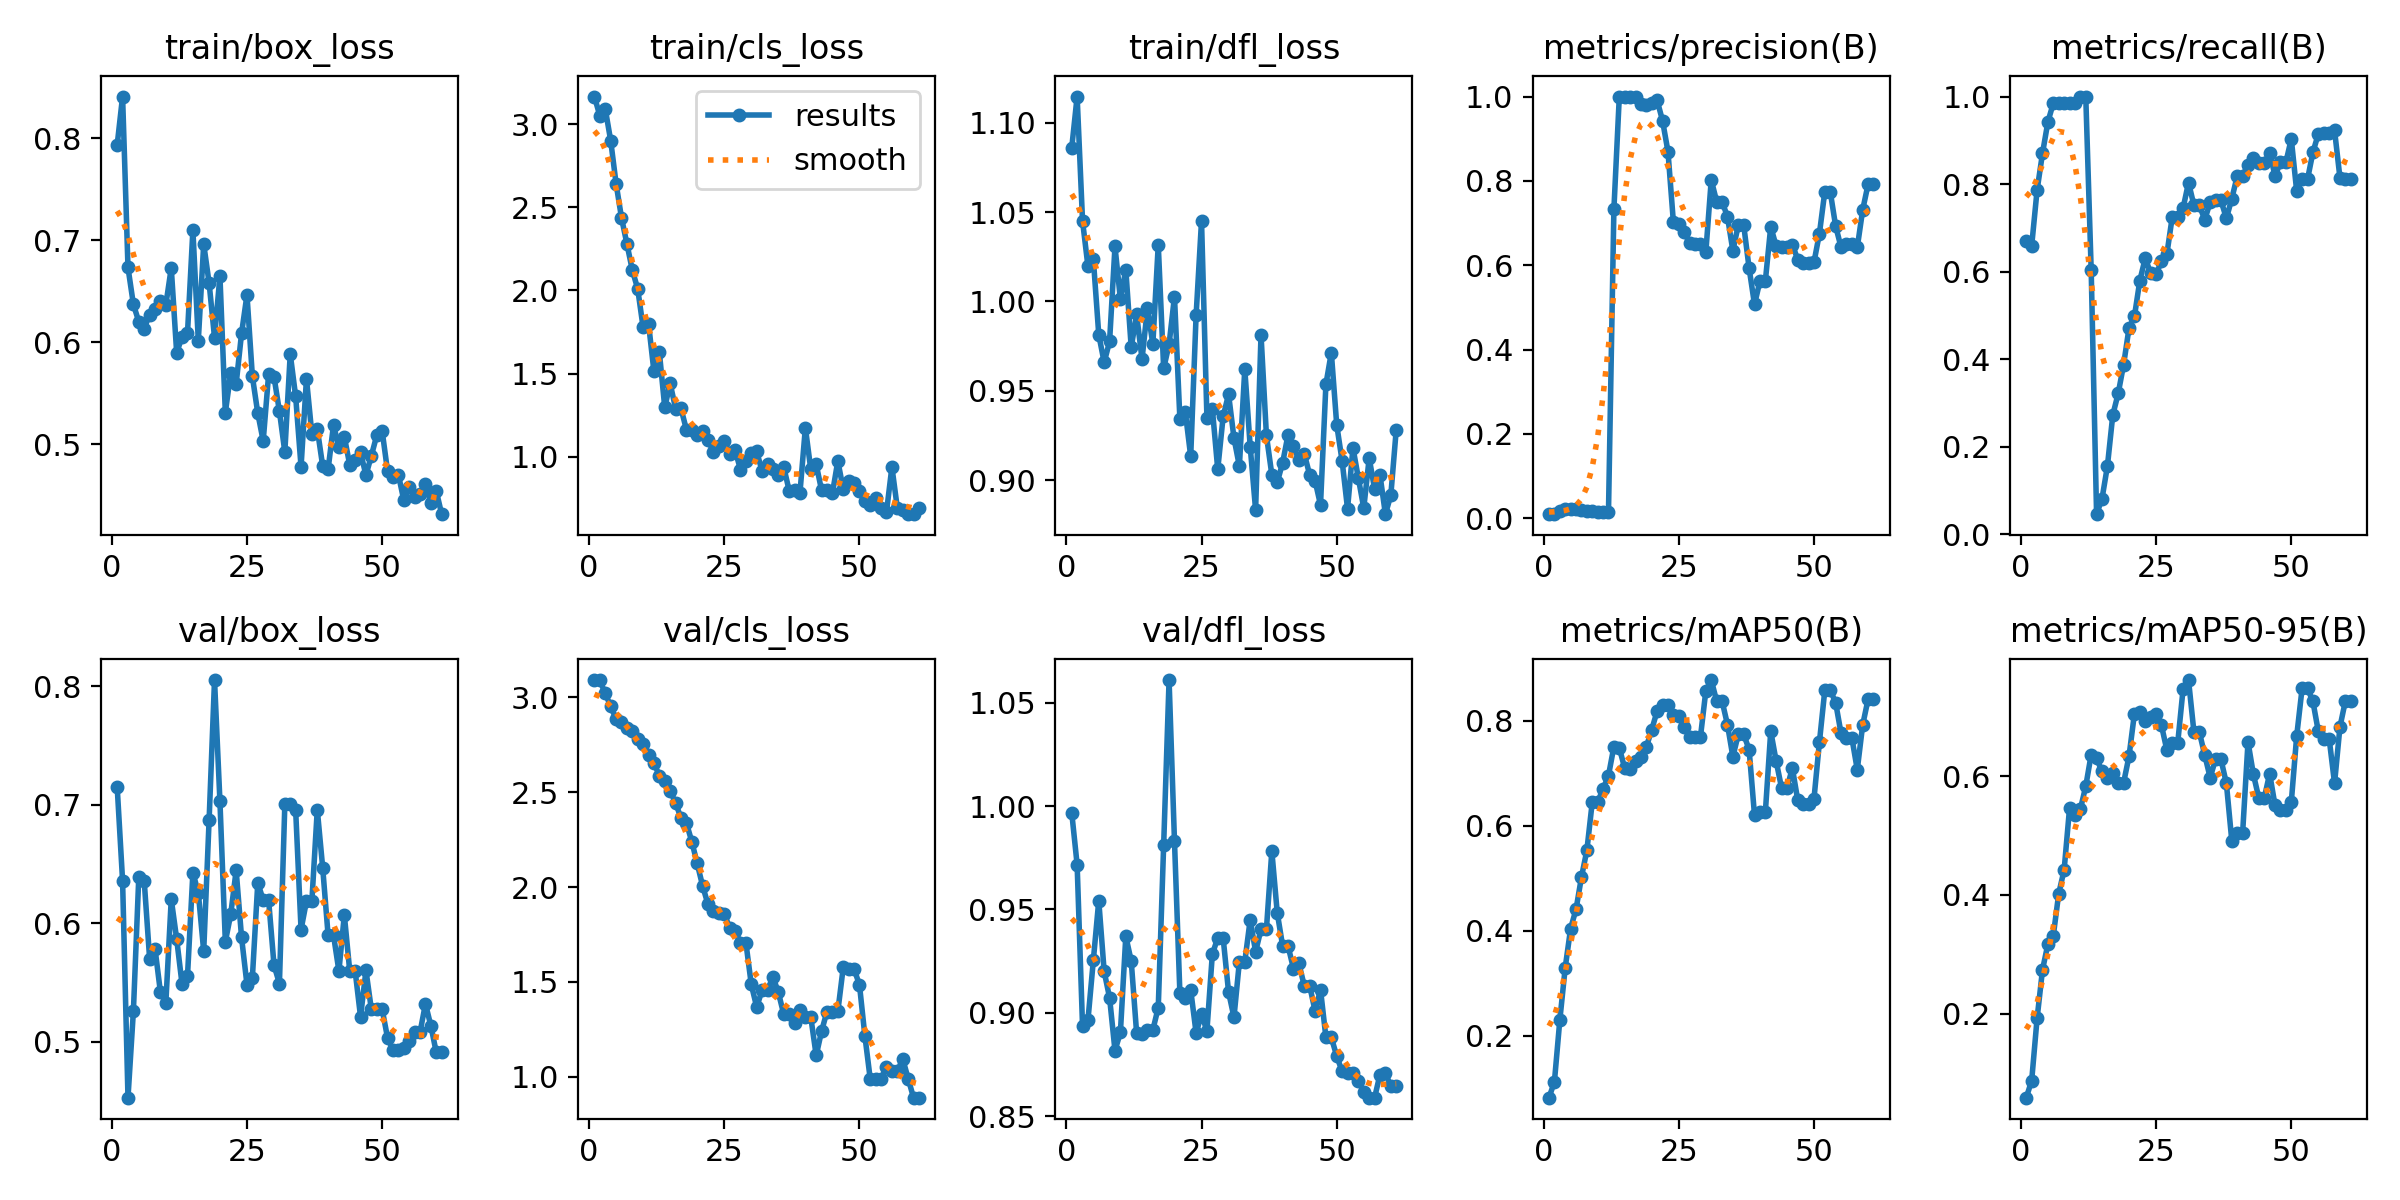
\includegraphics[width=0.48\textwidth]{training_results}
    }
    \subfigure[归一化混淆矩阵]{
        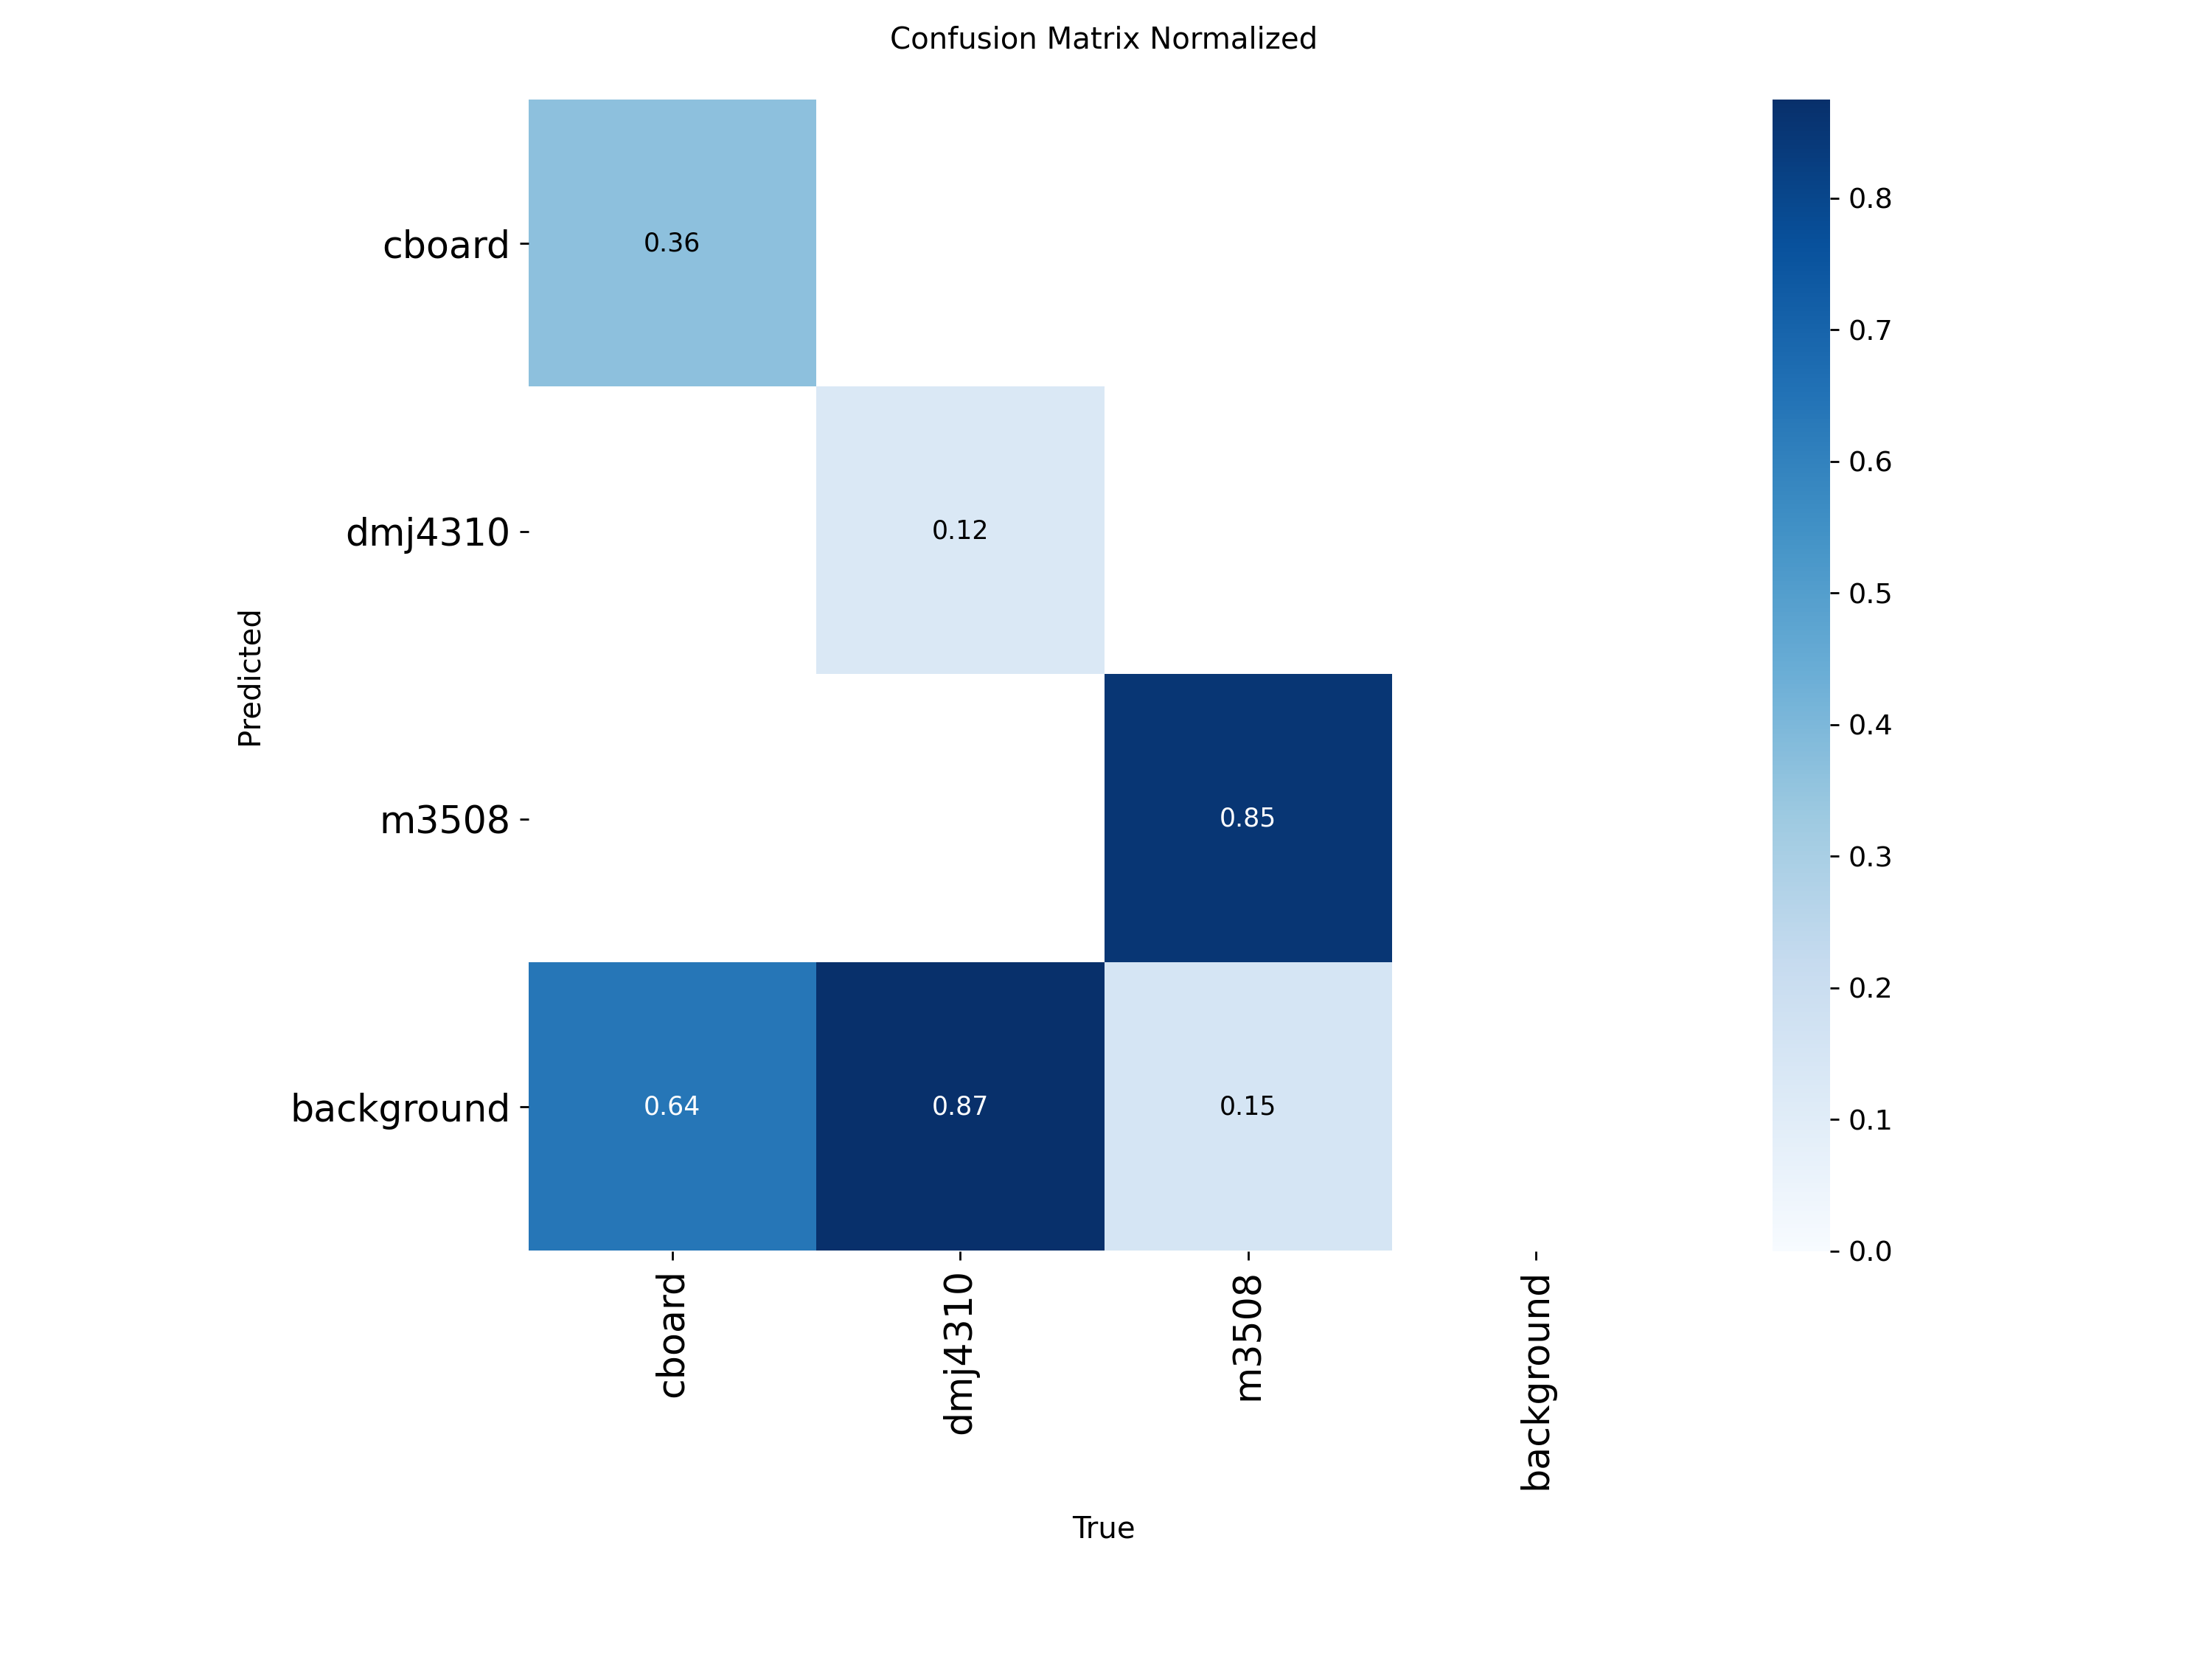
\includegraphics[width=0.48\textwidth]{confusion_matrix_normalized}
    }
    \caption{模型训练结果与类别区分情况}
    \label{fig:training}
\end{figure}

从图~\ref{fig:training} 可以看到，模型在前半段训练中提升很快，第 31 轮取得了较好的综合指标。后续指标存在一定波动，这与当前样本量偏小有关。对项目现阶段而言，这组结果足以支撑闭环演示；若要进入更稳定的长期使用，则需要继续补充不同角度、遮挡、反光和复杂背景下的样本。

\begin{figure}[H]
    \centering
    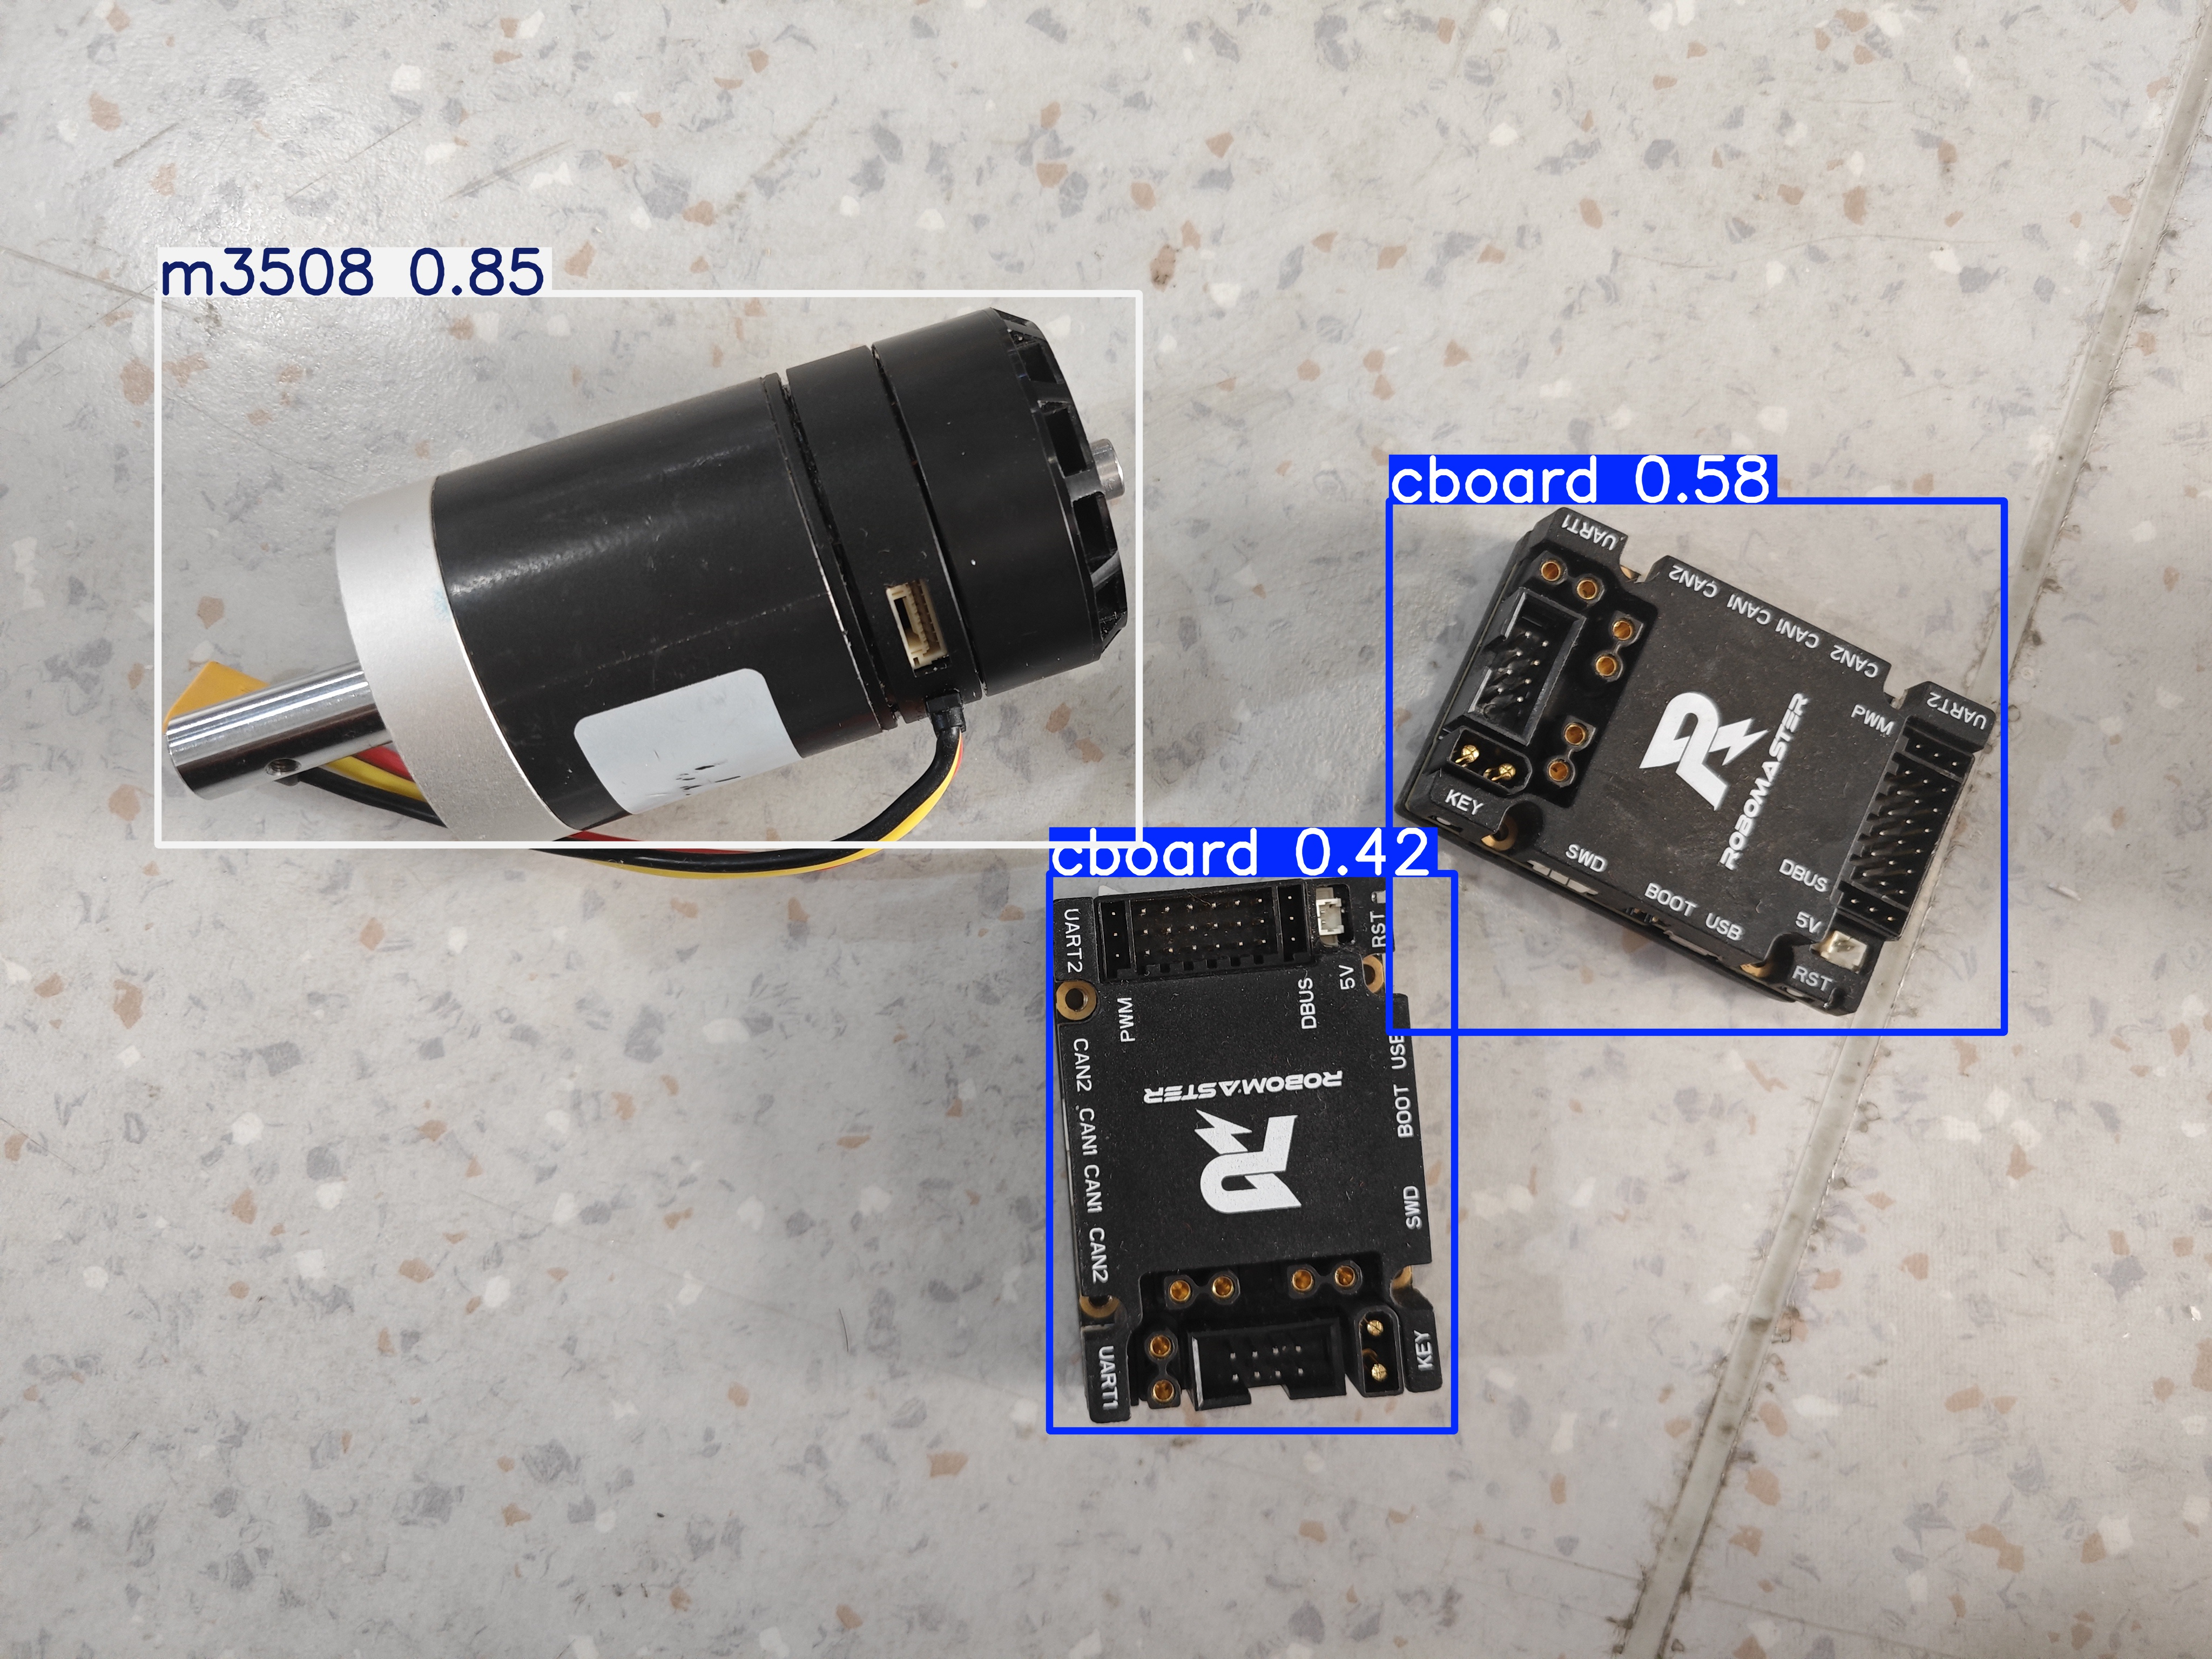
\includegraphics[width=0.72\textwidth]{prediction_example}
    \caption{单图物资检测与计数结果示例}
    \label{fig:prediction}
\end{figure}

图~\ref{fig:prediction} 对应的计数输出为 \code{cboard: 2}、\code{m3508: 1}。在系统流程中，这类计数不会停留在“画框展示”层面，而是会被客户端保存为前态或后态计数字典，随后参与库存差分。也就是说，模型输出已经和业务动作连在一起。

\section{系统亮点}

\subsection{客户端不再依赖 ROS2}

项目中一个很实用的改动，是把客户端从 ROS2 包改成独立 Python 程序。这样树莓派端只需要能运行摄像头、OpenCV 和 \code{tkinter}，不需要处理 ROS2 安装、工作空间编译和跨机器节点发现。服务端仍然保留 ROS2，客户端则用 TCP 接入，两边各自承担适合自己的复杂度。

\subsection{身份识别前置}

很多物资登记系统的问题不在数量，而在责任链断裂。本项目把人脸识别放在物资识别之前，并要求只有唯一已知人脸才能继续流程。后续 CSV 里的每一条记录都带有操作者姓名、操作时间和物资数量，查问题时不需要再反推“这次是谁登记的”。

\subsection{前后差分代替手工填数}

用户不需要手动输入“拿了几个、还了几个”，只要按流程拍摄前后两张图。系统根据两次 YOLO 计数自动拆分入库和出库条目。这个思路把视觉识别和库存管理连接起来，比单纯输出检测框更贴近实际使用。

\subsection{看板让结果可检查}

CSV 文件适合调试，但不适合展示。Web 看板补上了这一环：它把流水记录转换成当前库存、低库存提示、最近操作和单物资历史。老师或同学在演示时不必打开代码或 CSV，就能看到系统是否真的完成了记录闭环。

\section{不足与后续改进}

项目已经跑通主链路，但仍有不少可以继续打磨的地方。首先，物资检测目前只覆盖三类目标，数据集也偏小；下一步应优先扩充样本，特别是强反光、遮挡、相似背景和密集摆放场景。其次，人脸库成员较少，光照和姿态变化还需要更充分测试。第三，CSV 适合课程阶段，但如果要多人长期使用，后续应迁移到数据库，并补充账号权限、记录回滚和异常审核能力。

自动化程度也还有提升空间。当前前态物资图由用户手动点击抓拍，这是为了稳定演示而做的取舍。后续可以在预览端加入更可靠的画面稳定检测或固定支架提示，在保证不误拍的前提下减少用户操作步骤。

\section{总结}

本项目完成了一套从图像采集到库存展示的分布式智能物资管理系统。它的价值不只在于 YOLO 能识别三类物资，也在于把识别、人脸门控、TCP 通信、库存差分、CSV 落盘和 Web 看板串成了一个完整流程。当前实现已经证明“轻量客户端 + 集中式服务端 + 本地可视化看板”的路线适合课程项目，也为后续扩展更多物资类别、数据库存储和更自动化的端侧交互留下了清晰接口。

\newpage
\begin{thebibliography}{9}
    \addcontentsline{toc}{section}{参考资料}
    \bibitem{repo} 本项目代码仓库中的 \code{README.md}、\code{client/README.md}、\code{server/README.md}、\code{docs/project\_plan.md} 与 \code{docs/client\_server\_handoff\_2026-04-27.md}。
    \bibitem{ultralytics} Ultralytics Docs. \url{https://docs.ultralytics.com/}
    \bibitem{ros2} ROS 2 Humble Documentation. \url{https://docs.ros.org/en/humble/}
    \bibitem{face} face\_recognition Documentation. \url{https://face-recognition.readthedocs.io/en/latest/}
\end{thebibliography}

\end{document}
